\section{MOS gate verification}\label{gate_verify}
Now we have to verify that we don have relevant leakage on the gate with the thresholds and doping values we've set.

For that we use the formulas from \autoref{sub_threshold_leakage}

We can now plot multiple leakages for N- and P-channel transistors with a gate oxide thickness\footnote{See simulation/gate.wxmx} and with a surface concentration of $1e16\frac{1}{cm^3}=1e22\frac{1}{m^3}$ each
\begin{figure}[H]
	\centering
	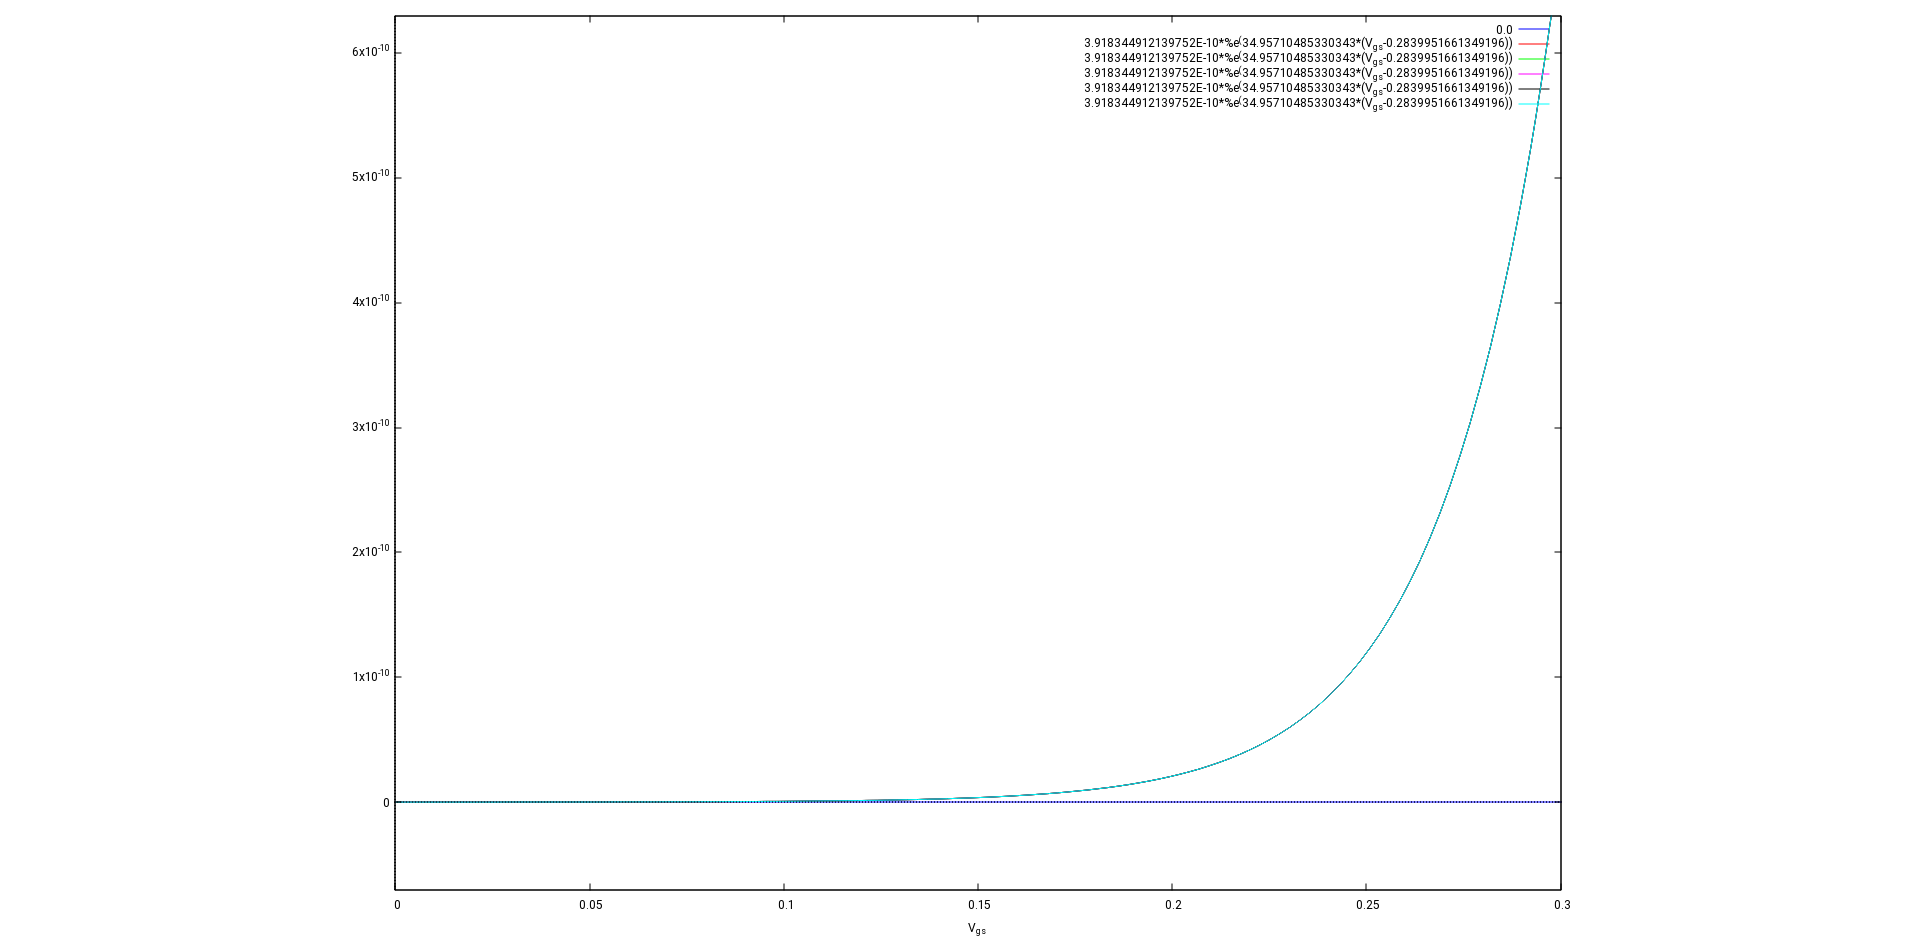
\includegraphics[width=\textwidth]{subthreshold_leagage.png}
	\caption{Subthreshold leakage plot(in Ampere)}
	\label{leagage_currents}
\end{figure}
In \autoref{leagage_currents} we see that with our gate oxide thickness this is really no problem, as we had expected.
From 0V up to 5V and further there is basically no leakage on the gate from the sub threshold current with $V_{Tn} \approx 0.39V$ and $V_{Tp} \approx -0.30V$.
That's good enough, as we will see in \autoref{nmos_dimensioning} and \autoref{pmos_dimensioning}.
There is actually a reduction of current when reaching the threshold because of the inversion of the capacity in the depletion zone\footnote{\url{https://people.eecs.berkeley.edu/~hu/Chenming-Hu_ch5.pdf}}, but I didn't include this into the calculation, because "TL;DR".
It's a TODO for release 2.1 of this process which will go sub $1 \mu m$